% LLM_course_slides.tex
% Cours de Traitement du Langage Naturel (NLP)

\documentclass[aspectratio=169]{beamer}
\usepackage[utf8]{inputenc}
\usepackage[T1]{fontenc}
\usepackage[french]{babel}
\usepackage{graphicx}
\usepackage{amsmath}
\usepackage{xcolor}
\usepackage{listings}
\usepackage{hyperref}
\usepackage{tikz}
\usepackage{booktabs}

% Thème Beamer
\usetheme{Madrid}
\usecolortheme{default}
\setbeamertemplate{navigation symbols}{}
\setbeamertemplate{footline}[frame number]

% Informations du titre
\title{Traitement du Langage Naturel (NLP) \\ \large{Des fondamentaux aux modèles de langage avancés}}
\author{Florian Valade}
\institute{Université Gustave Eiffel}
\date{\today}

\begin{document}

% Slide de titre
\begin{frame}
    \titlepage
\end{frame}

% Slide 2: Les entreprises d'IA
\begin{frame}{L'écosystème des entreprises d'IA}
    \begin{columns}
        \begin{column}{0.3\textwidth}
            \begin{center}
                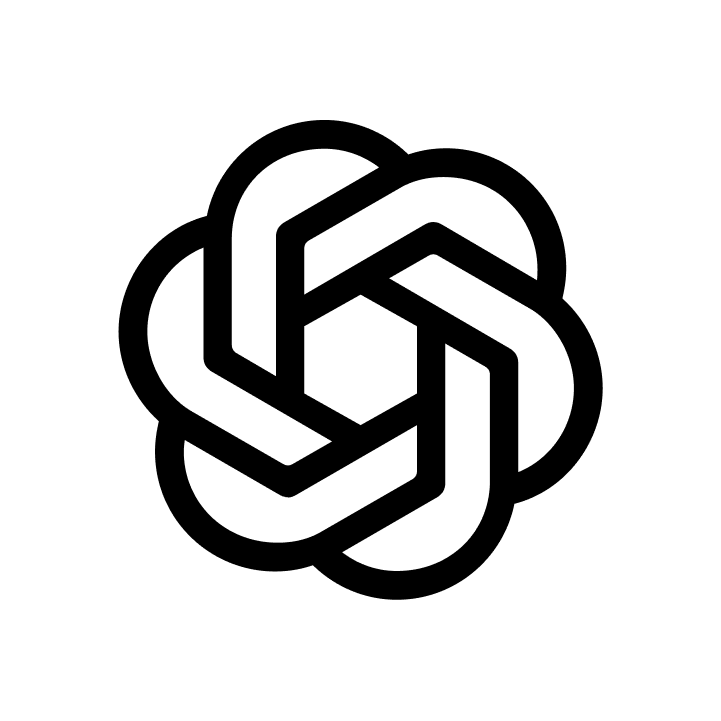
\includegraphics[width=0.3\textwidth]{images/openai.png} 
                \\ OpenAI (ChatGPT, GPT-4)
                        
                \vspace{0.5cm}
                
\includegraphics[width=0.3\textwidth]{images/anthropic.png}
                \\ Anthropic (Claude)
            \end{center}
        \end{column}
        \begin{column}{0.3\textwidth}
            \begin{center}
                
\includegraphics[width=0.3\textwidth]{images/mistral.png} 
                \\ Mistral AI
                
                \vspace{0.5cm}
                
                
\includegraphics[width=0.3\textwidth]{images/gemini.png} 
                \\ Google (Gemini)
                
                %\vspace{0.5cm}
                
                %\includegraphics[width=0.2\textwidth]{images/Meta_lockup_positive primary_RGB.png} 
                %\\ Meta (LLaMA)
            \end{center}
        \end{column}
        \begin{column}{0.3\textwidth}
                
\includegraphics[width=0.5\textwidth]{images/meta-color.png}
                \\ Meta (LLaMA)
        \end{column}
    \end{columns}
\end{frame}

% Slide 3: Capture d'écran de ChatGPT
\begin{frame}{Interface utilisateur des LLMs: ChatGPT}
    \begin{center}
        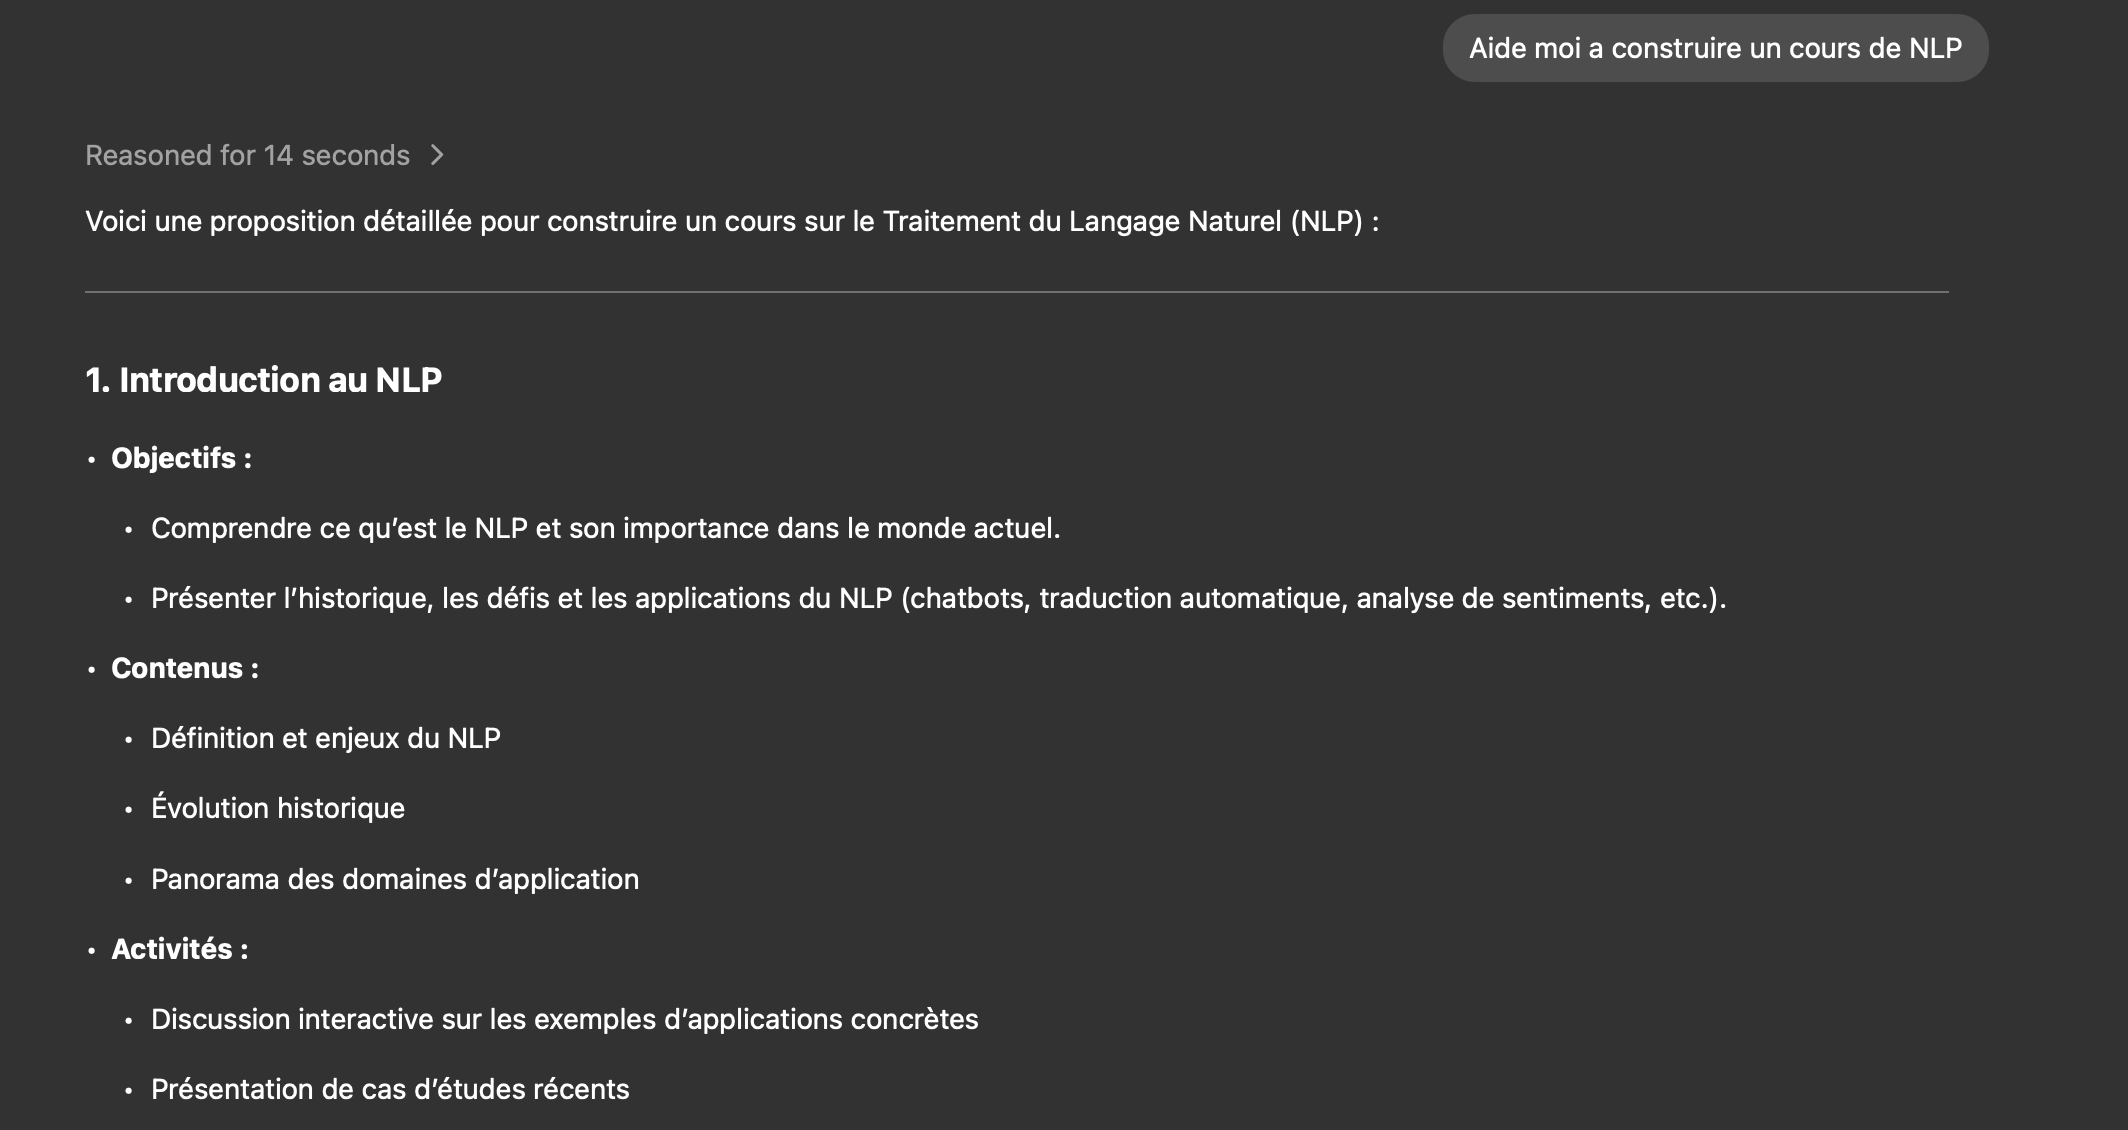
\includegraphics[width=0.6\textwidth]{images/chatbot.png} 
    \end{center}
    \begin{itemize}
        \item Interface conversationnelle intuitive
        \item Capacité à comprendre le contexte et les instructions
        \item Génération de réponses cohérentes et informatives
        \item Adaptabilité à différents types de requêtes
    \end{itemize}
\end{frame}

% Slide 4: Architecture de GPT
\begin{frame}{Ce qu'il y a derrière l'interface: Architecture des LLMs}
    \begin{columns}
        \begin{column}{0.6\textwidth}
            \begin{center}
                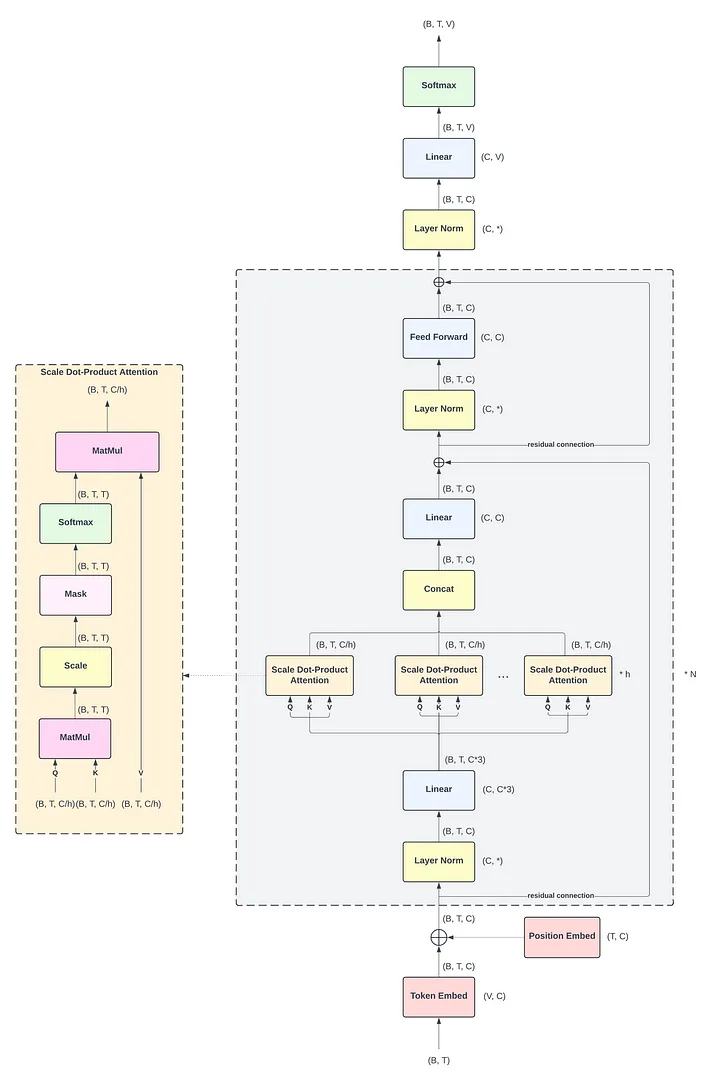
\includegraphics[width=0.5\textwidth]{images/gpt2.png}
            \end{center}
        \end{column}
        \begin{column}{0.4\textwidth}
            \begin{itemize}
                \item Architecture basée sur les Transformers
                \item Milliards de paramètres entraînés sur d'énormes corpus de texte
                \item Mécanisme d'attention pour capturer les dépendances à longue distance
                \item Apprentissage auto-supervisé (prédiction du token suivant)
            \end{itemize}
        \end{column}
    \end{columns}
\end{frame}

% Slide 5: Tokenisation
\begin{frame}{Rappel: La tokenisation}
    \begin{center}
        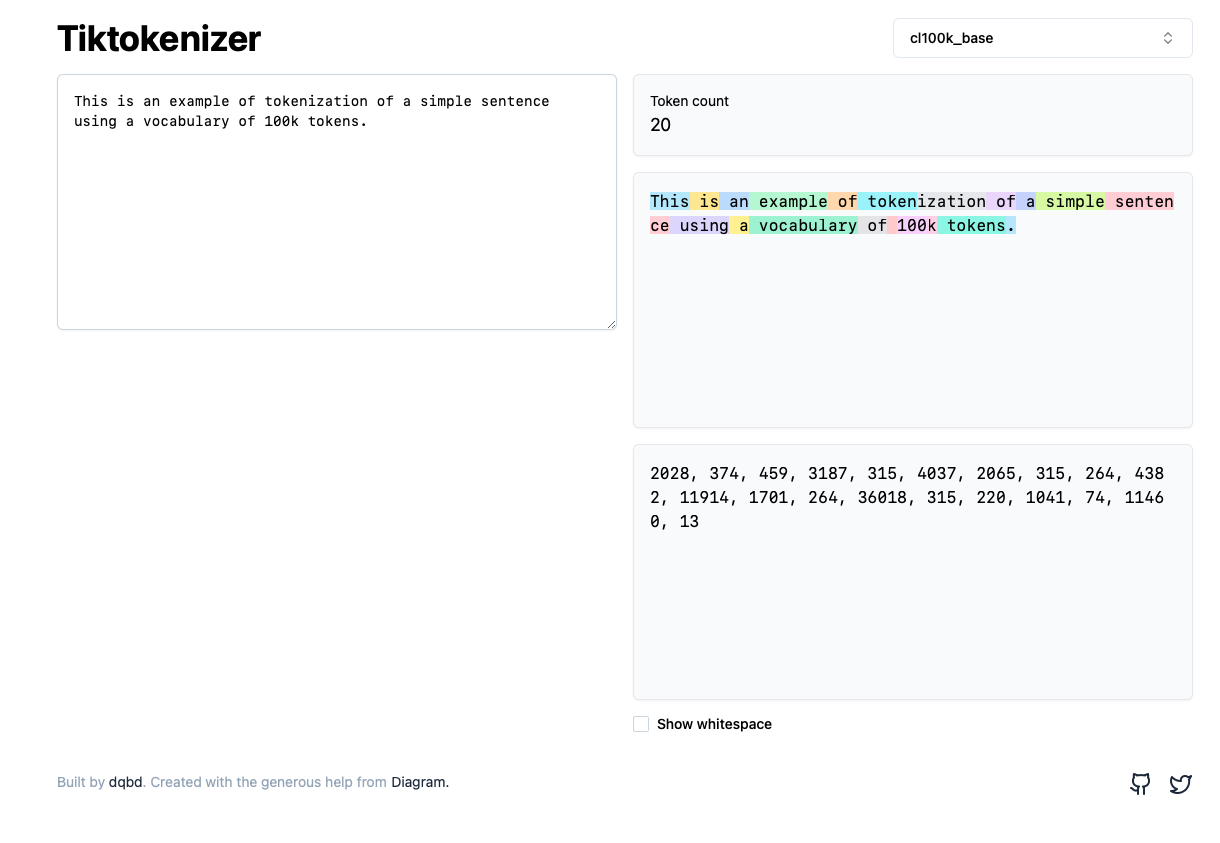
\includegraphics[width=0.5\textwidth]{images/tiktoken.png}
    \end{center}
    \begin{itemize}
        \item Les modèles de langage ne comprennent pas directement le texte
        \item Le texte est converti en séquences de tokens (unités de base)
        \item Différentes méthodes: par caractère, par mot, par sous-mot (BPE)
        \item Les tokens sont ensuite convertis en IDs numériques pour le modèle
    \end{itemize}
\end{frame}

% Slide 6: Génération de texte
\begin{frame}{Comment fonctionnent les LLMs: Génération de texte}
    \begin{center}
        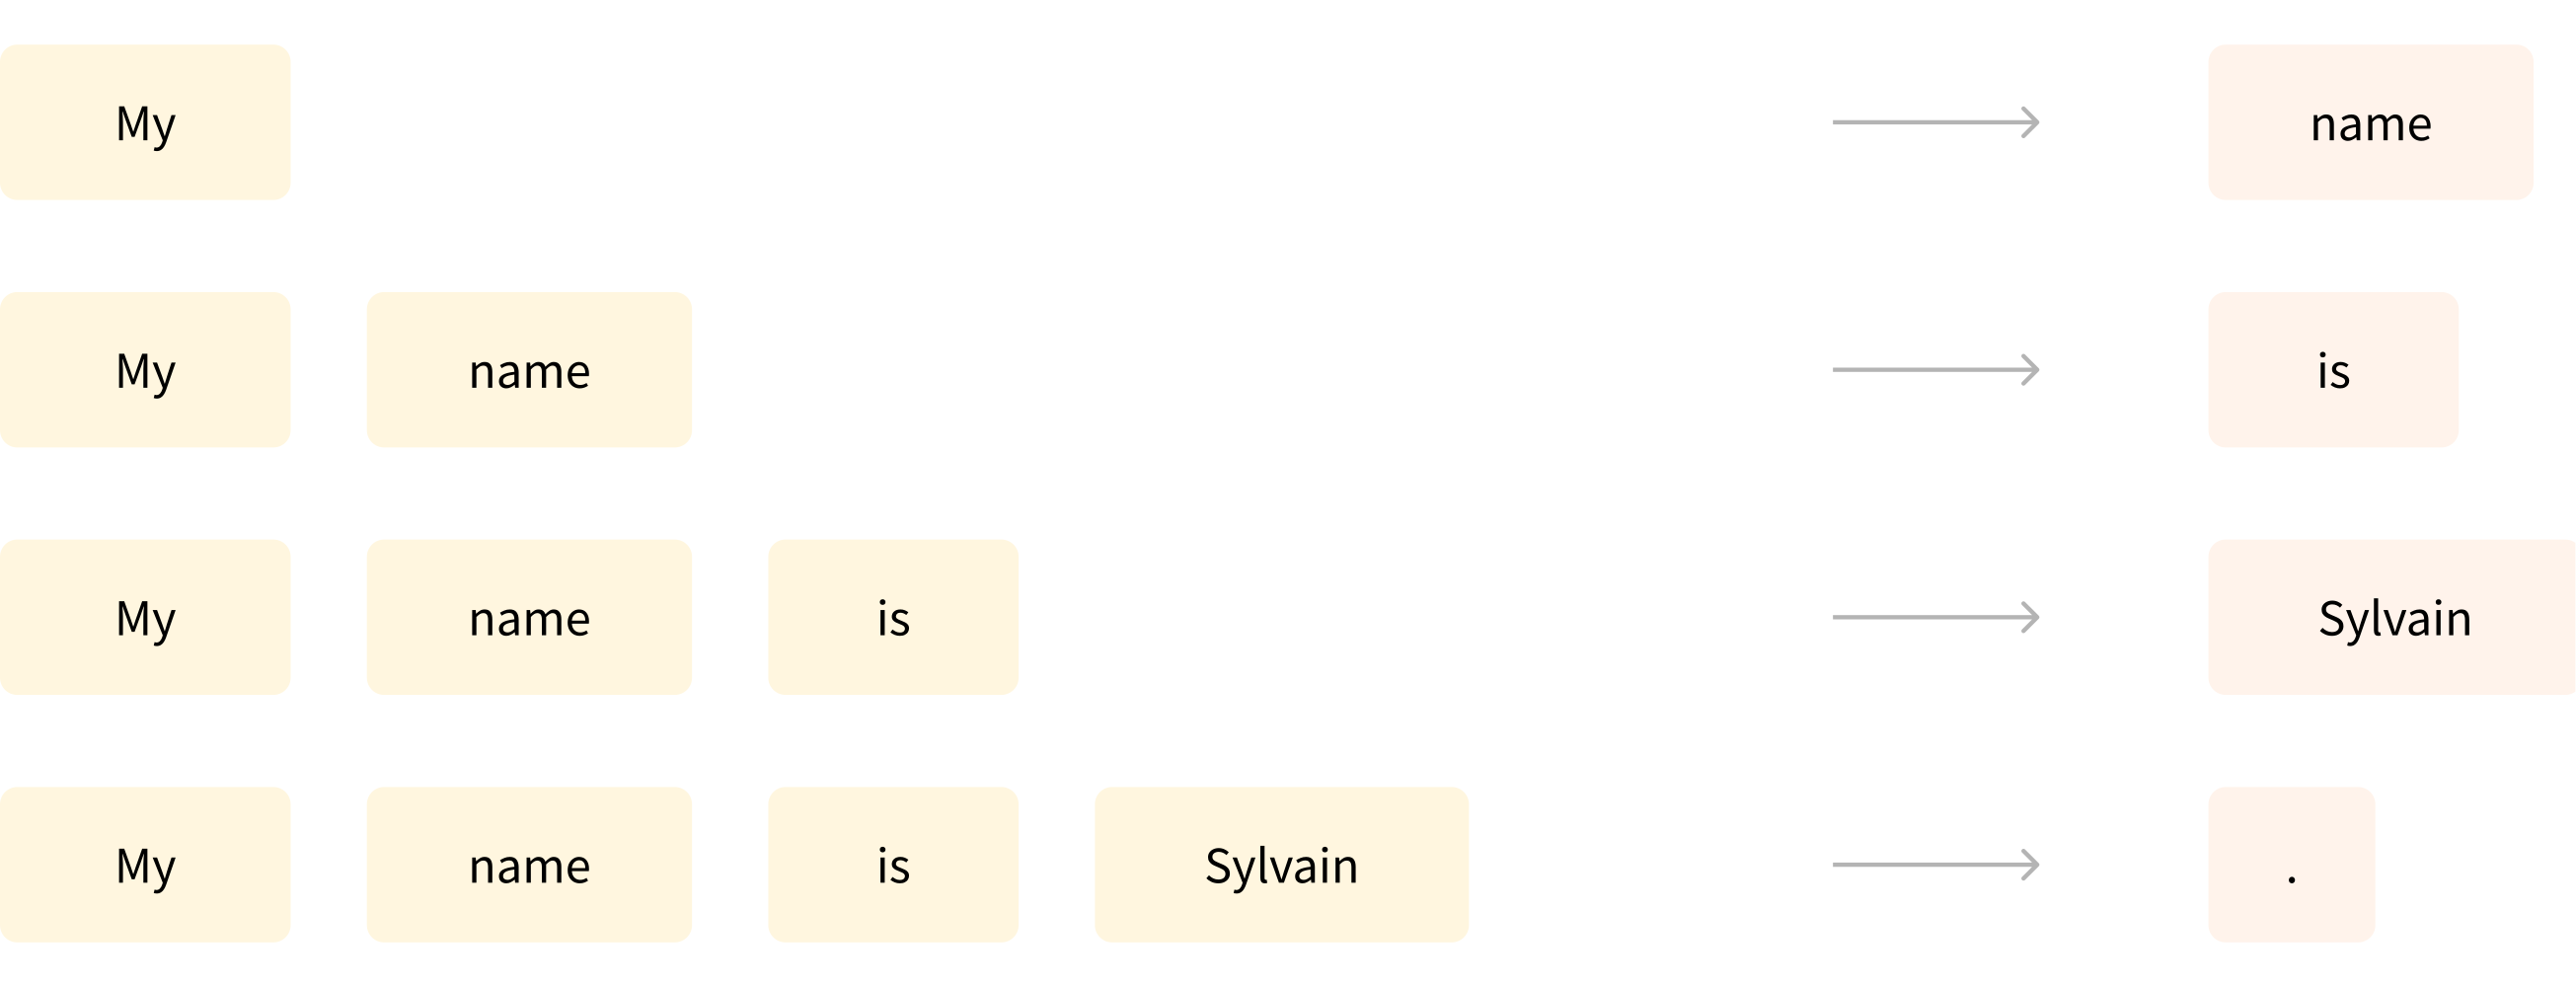
\includegraphics[width=0.5\textwidth]{images/causal_modeling.png} 
    \end{center}
    \begin{itemize}
        \item Génération auto-régressive: un token à la fois
        \item À chaque étape, le modèle prédit le token le plus probable suivant
        \item Le token prédit est ajouté au contexte pour la prédiction suivante
        \item Processus répété jusqu'à obtenir la réponse complète
    \end{itemize}
\end{frame}

% Slide 7: Titre pour la section Transformers
\begin{frame}{Les Transformers}
    \begin{center}
        \Large{\textbf{Architecture révolutionnaire en NLP}}
        
        \vspace{1cm}
        
        %\includegraphics[width=0.6\textwidth]{images/placeholder_transformer_overview.png} % Placeholder pour un aperçu des Transformers
    \end{center}
\end{frame}

% Slide 8: Architecture détaillée de GPT
\begin{frame}{Architecture détaillée des LLMs: Le modèle GPT}
    \begin{columns}
        \begin{column}{0.4\textwidth}
            \begin{center}
                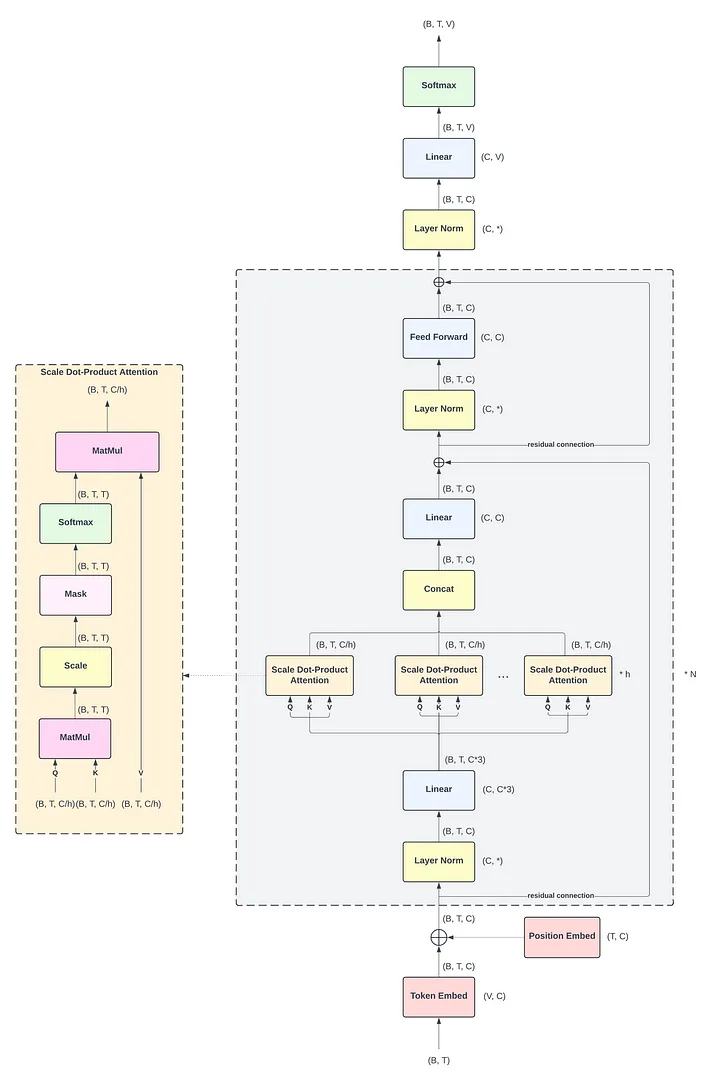
\includegraphics[width=0.7\textwidth]{images/gpt2.png}
                                
            \end{center}
        \end{column}
        \begin{column}{0.6\textwidth}
            \begin{itemize}
                \item \textbf{Embedding}: conversion des tokens en vecteurs denses
                \item \textbf{Positional encoding}: intégration de l'information de position
                \item \textbf{N blocs Transformer}: traitement contextuel profond
                \item \textbf{Layer normalization}: stabilise l'apprentissage
                \item \textbf{Connexions résiduelles}: facilite l'entraînement de réseaux profonds
                \item \textbf{Tête de classification}: prédit le token suivant
            \end{itemize}
        \end{column}
    \end{columns}
\end{frame}




% Slide 9: Architecture Encoder-Decoder
\begin{frame}{Architecture originale des Transformers: Encoder-Decoder}
    \begin{columns}
        \begin{column}{0.5\textwidth}
            \begin{center}
                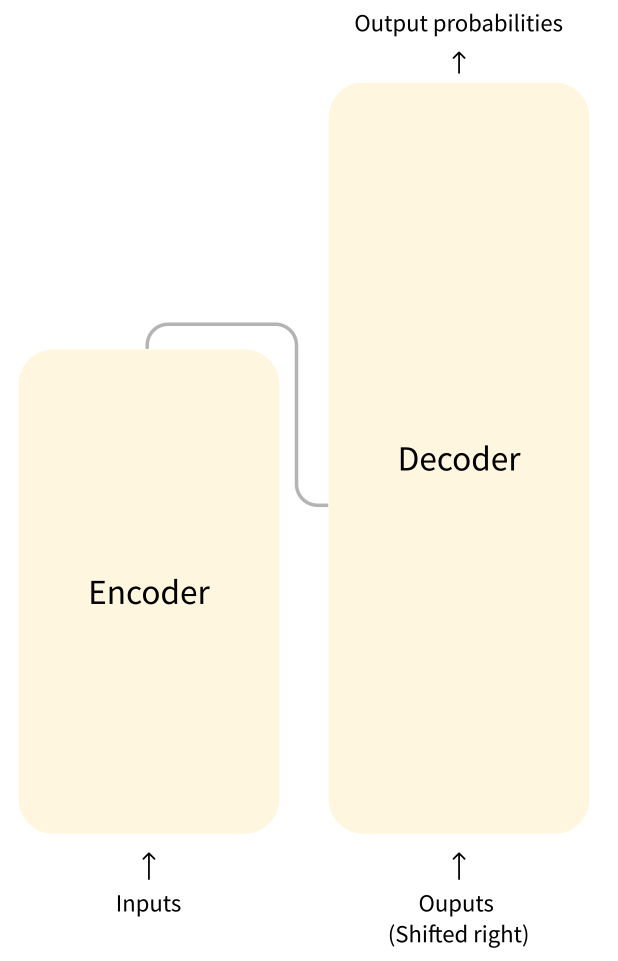
\includegraphics[width=0.6\textwidth]{images/encoder_decoder.png}
            \end{center}
        \end{column}
        \begin{column}{0.5\textwidth}
            \begin{itemize}
                \item Architecture présentée dans \textit{"Attention is All You Need"} (2017)
                \item \textbf{Encoder}: traite l'ensemble de la séquence d'entrée
                \item \textbf{Decoder}: génère la séquence de sortie token par token
                \item Parfaite pour la \textbf{traduction automatique}, où la taille de sortie est inconnue
                \item GPT utilise uniquement la partie \textbf{decoder} (auto-régressive)
                \item BERT utilise uniquement la partie \textbf{encoder} (bi-directionnelle)
            \end{itemize}
        \end{column}
    \end{columns}
\end{frame}

% Slide 9.5: Focus sur l'architecture GPT - Entrée
\begin{frame}{Focus sur l'entrée du modèle GPT}
    \begin{columns}
        \begin{column}{0.5\textwidth}
            \begin{center}
                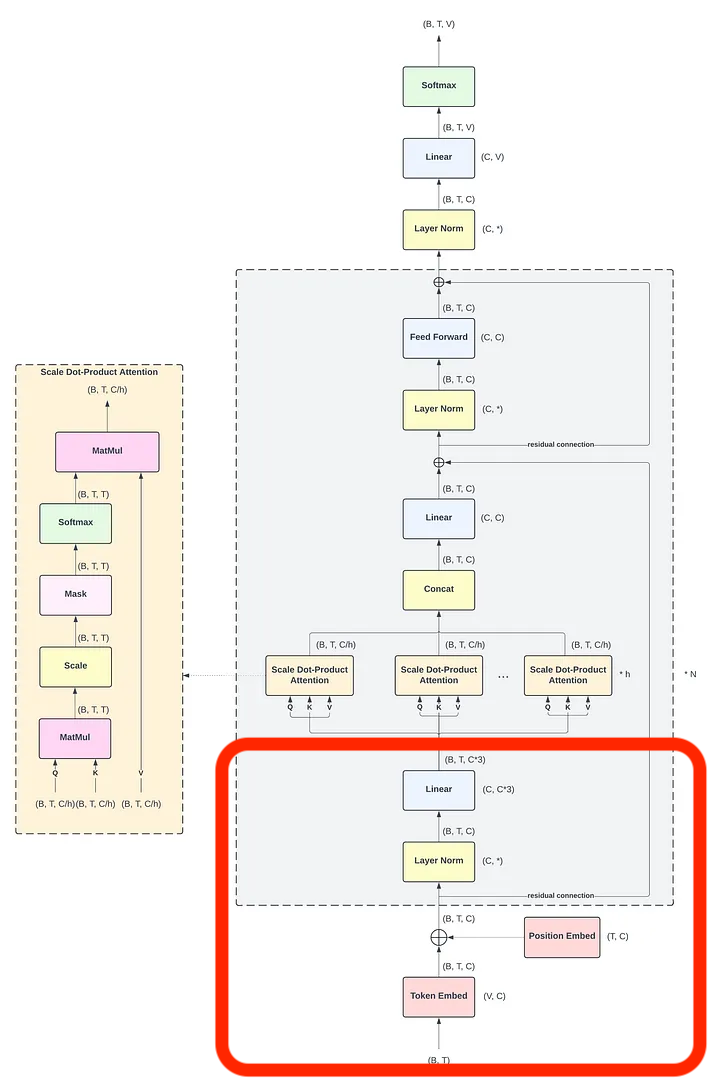
\includegraphics[width=0.5\textwidth]{images/gpt2_in.png}
            \end{center}
        \end{column}
        \begin{column}{0.5\textwidth}
            Plusieurs étapes :
            \begin{itemize}
                \item Tokenisation : Texte $\rightarrow$ Tokens $[context\_length]$
                \item Embedding : Tokens $\rightarrow$ Vecteurs $[context\_length, embedding\_dim]$
                \item Positional encoding : Vecteurs $\rightarrow$ Vecteurs $[context\_length, embedding\_dim]$
                \item Layer normalization : Vecteurs $\rightarrow$ Vecteurs $[context\_length, embedding\_dim]$
                \item Projections QKV : Vecteurs $\rightarrow$ Vecteurs $[context\_length, 3 \times embedding\_dim]$
            \end{itemize}
        \end{column}
    \end{columns}
\end{frame}

% Slide 10: Exemple de traitement d'une phrase
\begin{frame}{Du texte aux vecteurs: Tokenisation}
    \begin{center}
        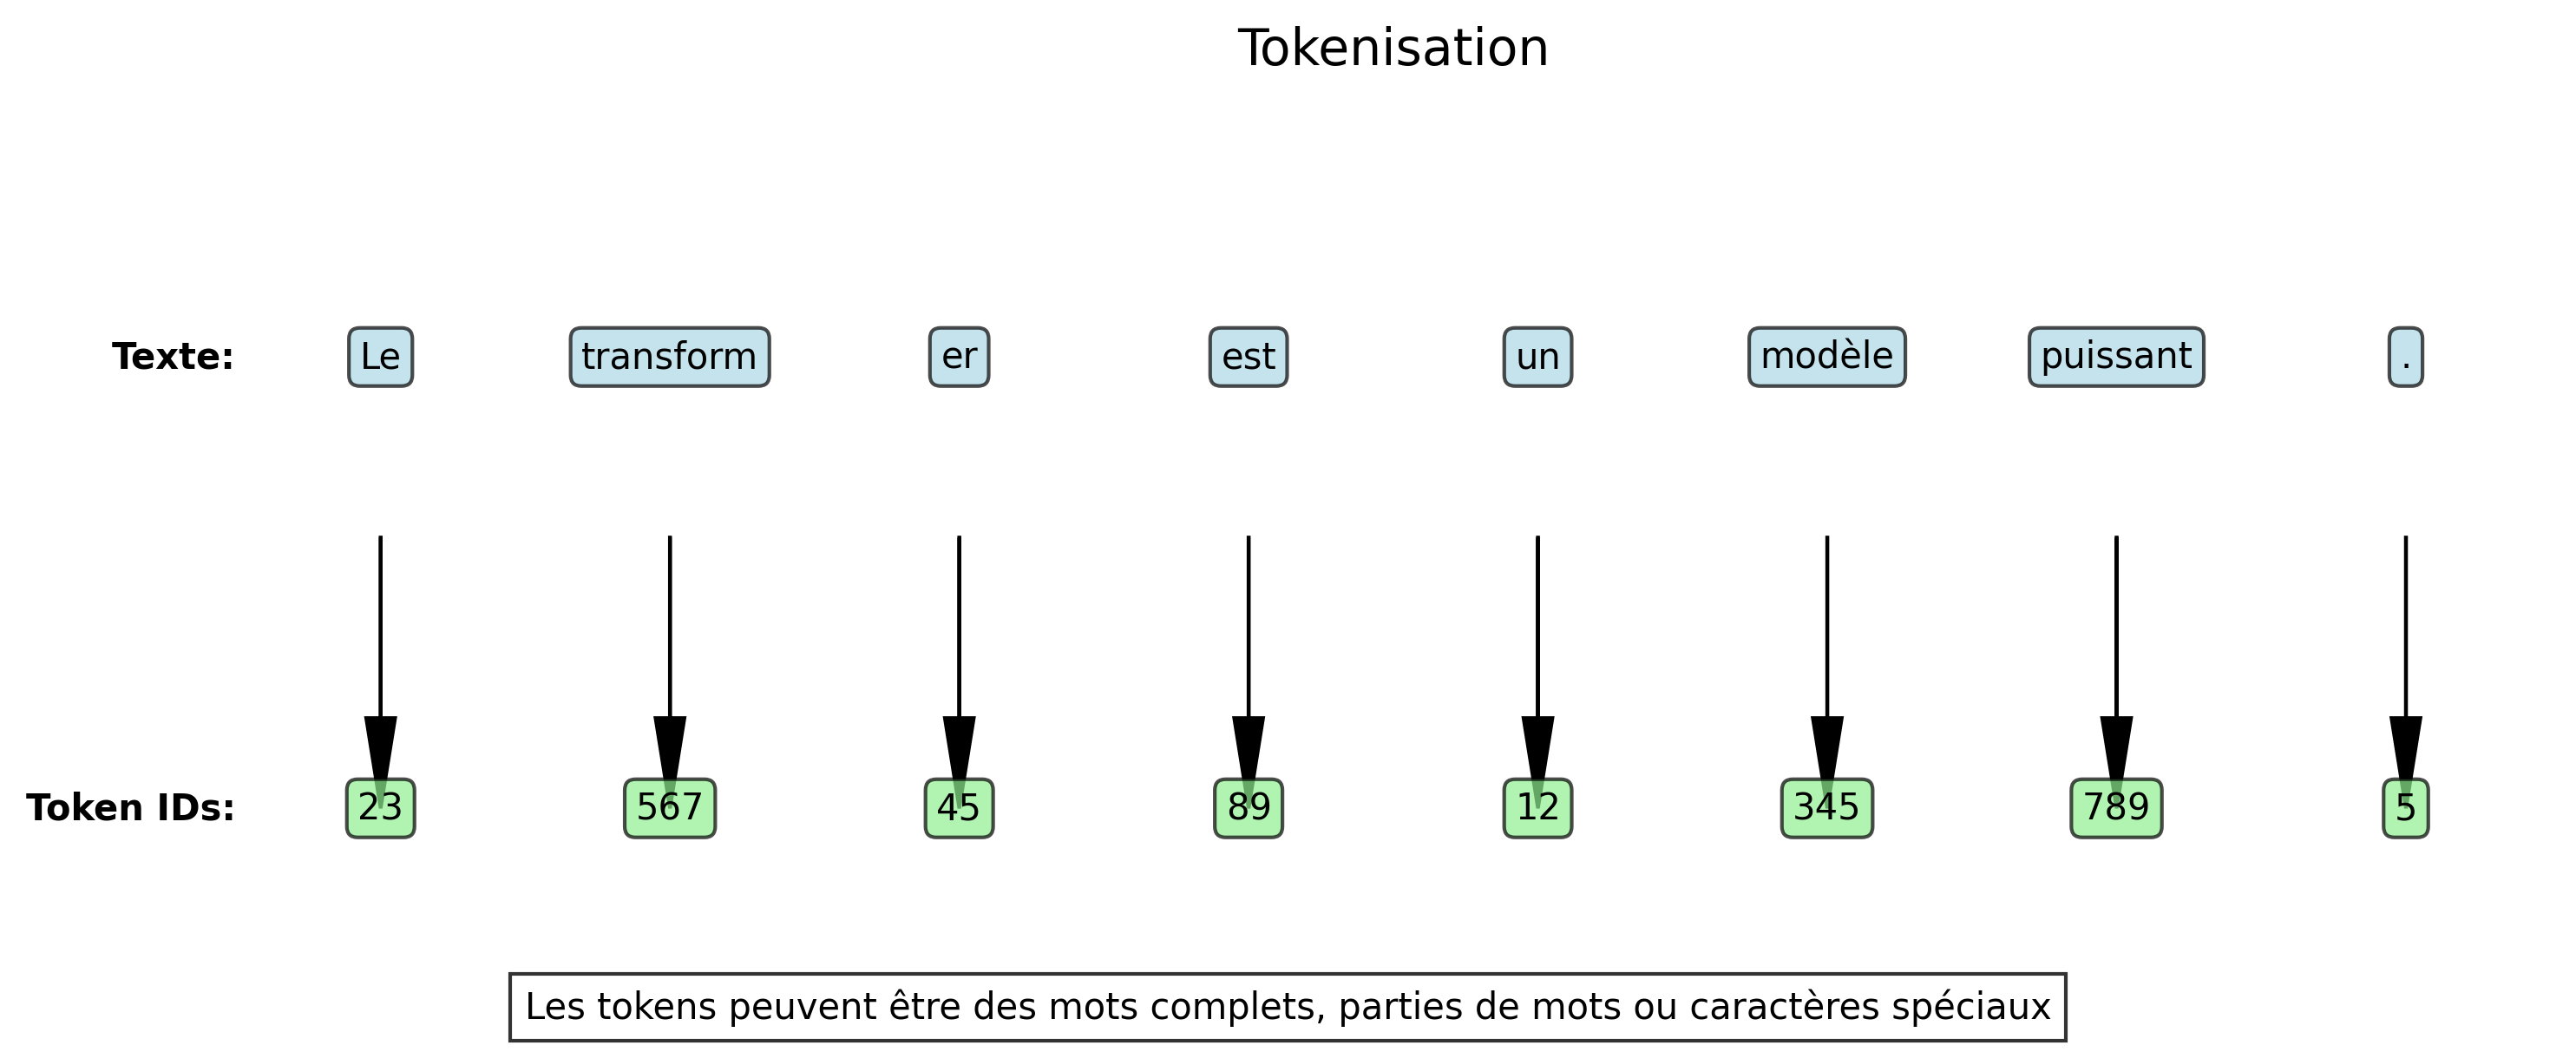
\includegraphics[width=0.8\textwidth]{images/generated/tokenization_process.png}
    \end{center}
    \begin{itemize}
        \item \textbf{Tokenisation}: découpage du texte en unités (tokens) que le modèle peut traiter
        \item Différentes méthodes: par caractère, par mot, par sous-mot (BPE)
        \item Les tokens sont ensuite convertis en IDs numériques pour le modèle
    \end{itemize}
\end{frame}

% Slide 11: Embedding
\begin{frame}{Embedding: Conversion des tokens en vecteurs}
    \begin{columns}
        \begin{column}{0.6\textwidth}
            \begin{center}
                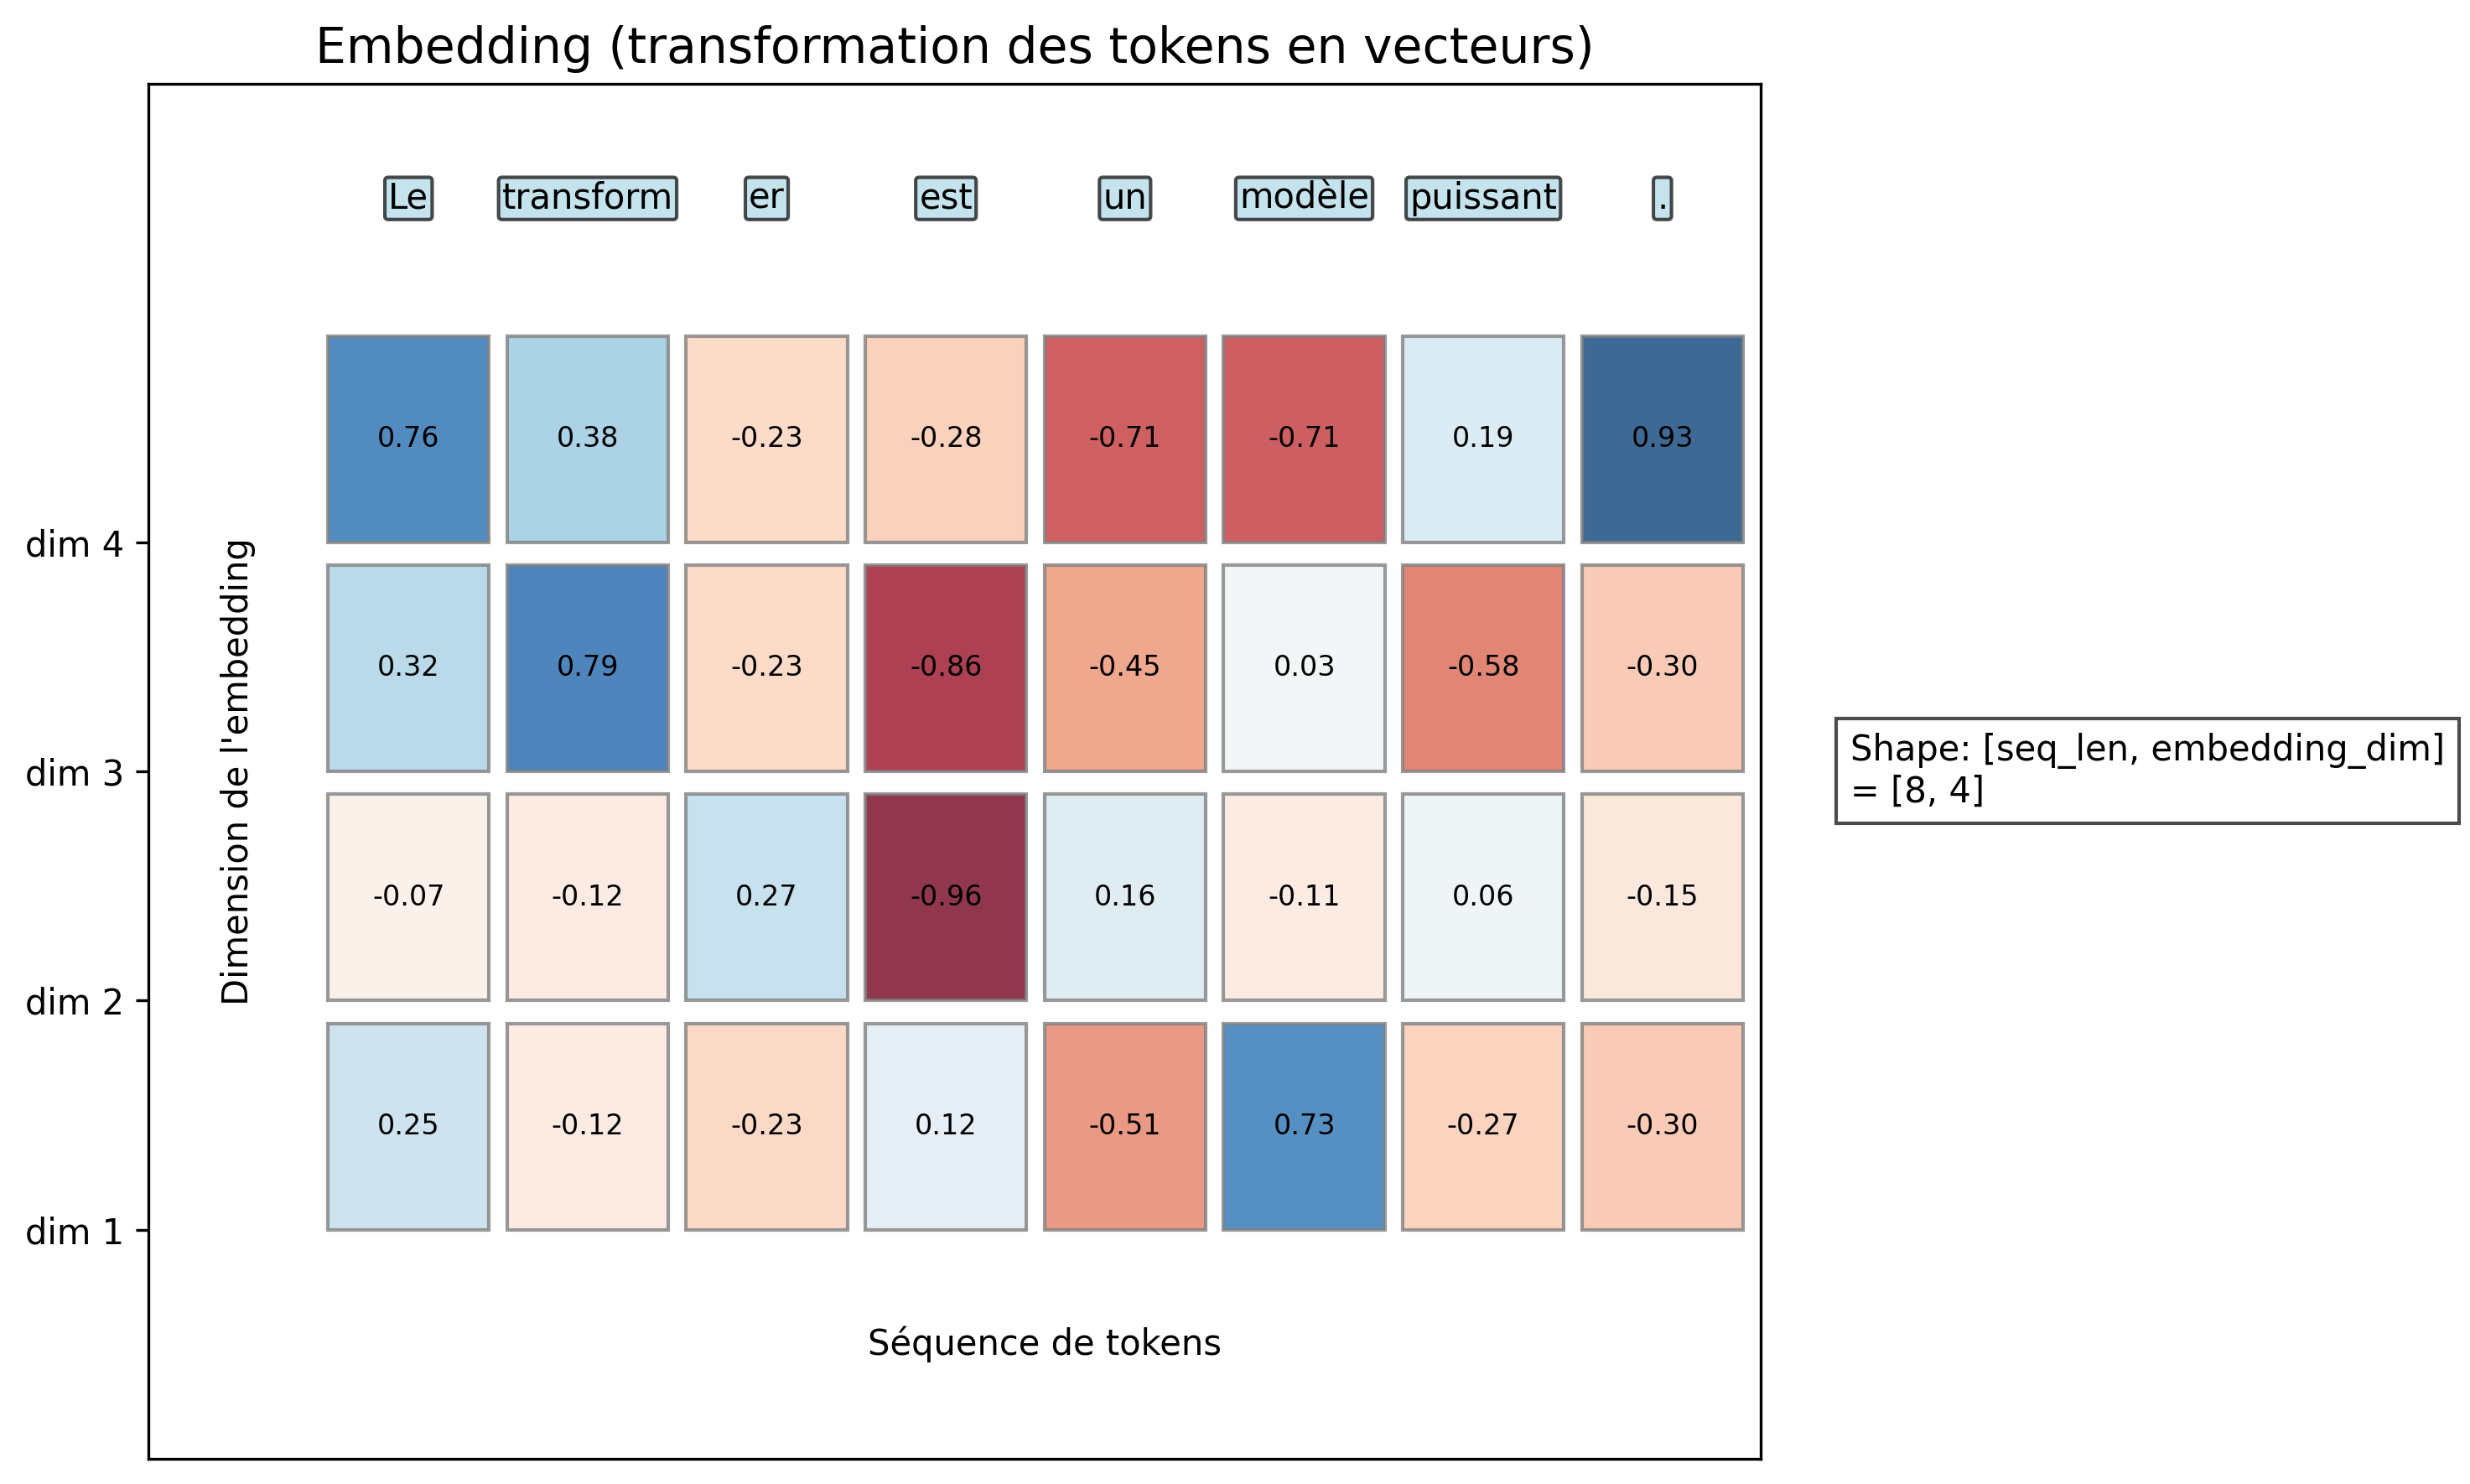
\includegraphics[width=\textwidth]{images/generated/embedding_process.png}
            \end{center}
        \end{column}
        \begin{column}{0.4\textwidth}
            \begin{itemize}
                \item \textbf{Embedding}: transformation des tokens en vecteurs de nombres réels
                \item Dimension d'embedding typique: 768 à 4096 selon la taille du modèle
                \item Les vecteurs capturent les relations sémantiques entre les tokens
                \item La matrice d'embedding est apprise lors de l'entraînement du modèle
            \end{itemize}
        \end{column}
    \end{columns}
\end{frame}

% Slide 12: Layer Normalization
\begin{frame}{Layer Normalization: Stabiliser l'apprentissage}

    \begin{align*}
        \hat{x} &= \frac{x - \mu}{\sigma} \\
        y &= \gamma \cdot \hat{x} + \beta
    \end{align*}
    \begin{itemize}
        \item $\mu$ et $\sigma$ sont les moyennes et écarts-types des vecteurs de token
        \item Normalise chaque vecteur de token indépendamment
        \item Réduit la covariance interne (shift covariate)
        \item Stabilise et accélère l'entraînement des réseaux profonds
        \item Paramètres apprenables $\gamma$ et $\beta$ pour préserver la capacité expressive
    \end{itemize}
\end{frame}

% Slide 13: Mécanisme d'attention
\begin{frame}{Le cœur du Transformer: L'attention}
    \begin{center}
        \begin{tikzpicture}[>=latex, node distance=1.5cm, scale=0.65, transform shape]
            % Title for QKV transformations
            \node[text width=12cm, align=center] at (6,1) {\textbf{Projections linéaires pour Query (Q), Key (K), Value (V)}};
            
            % Inputs
            \foreach \i in {1,...,4}
            {
                \node (Input-\i) at (0,-\i) {$x_\i$};
            }

            % Hidden Layer - Q
            \foreach \i in {1,...,3}
            {
                \node[draw, circle, minimum size=1cm] (Hidden-\i) at (3,{-\i*1.5+0.5}) {$f$};
            }
            \node at (3,0) {Q};

            % Inputs
            \foreach \i in {1,...,4}
            {
                \node (Input2-\i) at (6,-\i) {$x_\i$};
            }
            % Hidden Layer - K
            \foreach \i in {1,...,3}
            {
                \node[draw, circle, minimum size=1cm] (Hidden2-\i) at (9,{-\i*1.5+0.5}) {$f$};
            }
            \node at (9,0) {K};
            
            % Inputs
            \foreach \i in {1,...,4}
            {
                \node (Input3-\i) at (12,-\i) {$x_\i$};
            }
            % Hidden Layer - V
            \foreach \i in {1,...,3}
            {
                \node[draw, circle, minimum size=1cm] (Hidden3-\i) at (15,{-\i*1.5+0.5}) {$f$};
            }
            \node at (15,0) {V};
            
            % Draw connections from inputs to the hidden layer
            \foreach \i in {1,...,4}
            {
                \foreach \j in {1,...,3}
                {
                    \draw[->] (Input-\i) -- (Hidden-\j);
                    \draw[->] (Input2-\i) -- (Hidden2-\j);
                    \draw[->] (Input3-\i) -- (Hidden3-\j);
                }
            }

        \end{tikzpicture}
    \end{center}
    \begin{itemize}
        \item \textbf{Query (Q)}, \textbf{Key (K)}, \textbf{Value (V)}: projections différentes du même input
        \item Score d'attention: $\text{Attention}(Q, K, V) = \text{softmax}\left(\frac{QK^T}{\sqrt{d_k}}\right)V$
        \item Permet de capturer différents types de relations entre tokens
        \item Query représente la question, Key représente les réponses possibles, Value représente les réponses
    \end{itemize}
\end{frame}

% Slide 14: Récapitulation QKV
\begin{frame}{Récapitulation: Les matrices Query, Key et Value}
    \begin{columns}
        \begin{column}{0.4\textwidth}
            \begin{center}
                %\includegraphics[width=\textwidth]{images/qkv.png}
                \begin{tikzpicture}[scale=0.9]
                    % Matrices
                    \draw[fill=yellow!20] (0,0) rectangle (1.5,3) node[pos=.5] {$Q$};
                    \draw[fill=red!20] (2,0) rectangle (3.5,3) node[pos=.5] {$K$};
                    \draw[fill=green!20] (4,0) rectangle (5.5,3) node[pos=.5] {$V$};
                    
                    % Dimensions
                    \draw[<->] (0,-0.5) -- (1.5,-0.5) node[midway, below] {$d_{emb}$};
                    \draw[<->] (2,-0.5) -- (3.5,-0.5) node[midway, below] {$d_{emb}$};
                    \draw[<->] (4,-0.5) -- (5.5,-0.5) node[midway, below] {$d_{emb}$};
                    \draw[<->] (-0.5,0) -- (-0.5,3) node[midway, left] {$C_{len}$};
                \end{tikzpicture}
            \end{center}
        \end{column}
        \begin{column}{0.6\textwidth}
            \begin{itemize}
                \item Trois matrices de taille [contexte, embedding] ou une matrice de taille [contexte, 3 × embedding]
                \item \textbf{Queries (Q)} : Représentent ce que recherche chaque token
                \begin{itemize}
                    \item "Quelles informations sont importantes pour moi?"
                \end{itemize}
                \item \textbf{Keys (K)} : Encapsulent les informations disponibles dans chaque token
                \begin{itemize}
                    \item "Voici les informations que je peux fournir"
                \end{itemize}
                \item \textbf{Values (V)} : Contiennent les informations effectives à combiner
                \begin{itemize}
                    \item "Voici mon contenu qui sera utilisé pour la sortie"
                \end{itemize}
                \item Les scores d'attention (QK$^T$) déterminent quelles valeurs (V) sont pertinentes
            \end{itemize}
        \end{column}
    \end{columns}
\end{frame}


% Slide 15: Introduction au mécanisme d'attention
\begin{frame}{Le mécanisme d'attention: Comprendre les relations contextuelles}
    \begin{columns}
        \begin{column}{0.5\textwidth}
            \begin{center}
                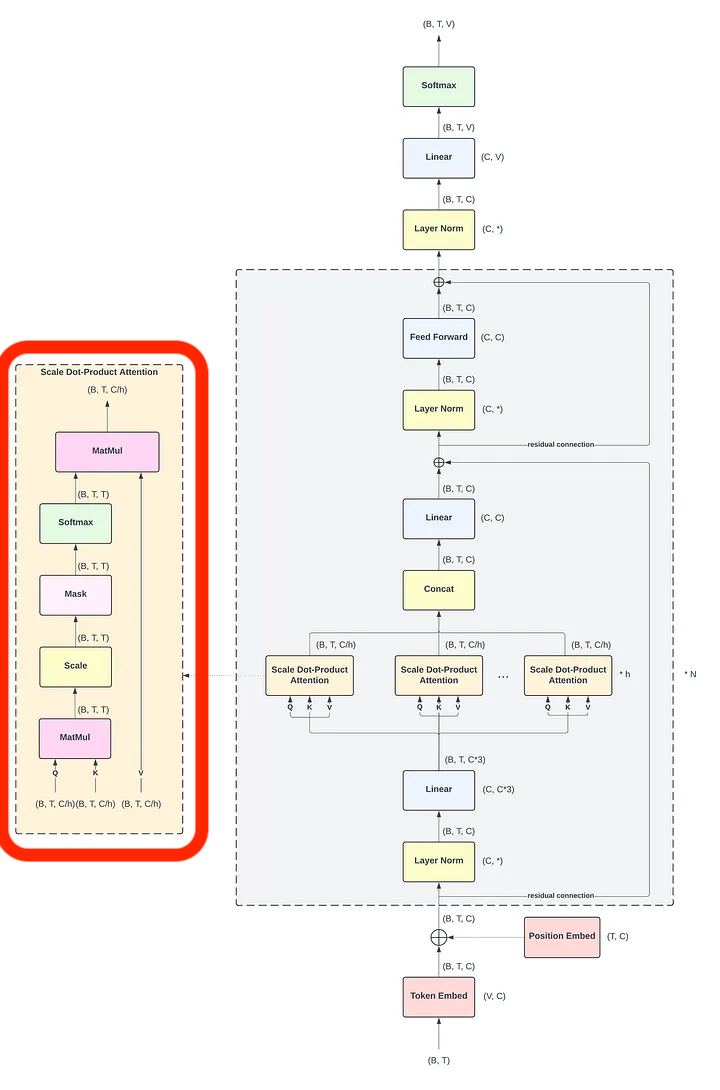
\includegraphics[width=0.5\textwidth]{images/gpt2_attn.png}
            \end{center}
        \end{column}
        \begin{column}{0.5\textwidth}
            \begin{itemize}
                \item L'attention est le \textbf{cœur des Transformers}
                \item Permet de \textbf{pondérer dynamiquement} l'importance de chaque token
                \item Capture les \textbf{dépendances à longue distance}
                \item Chaque token peut "prêter attention" à tous les tokens précédents
            \end{itemize}
        \end{column}
    \end{columns}
\end{frame}


% Slide 16: Scaled Dot-Product Attention
\begin{frame}{Scaled Dot-Product Attention}
    \begin{columns}
        \begin{column}{0.4\textwidth}
            \begin{center}
                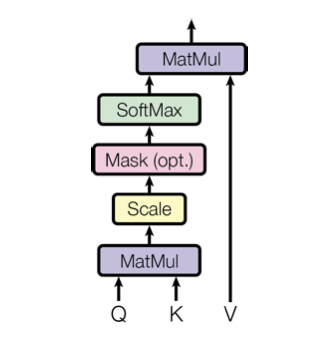
\includegraphics[width=\textwidth]{images/scaled_dot_attn.png}
            \end{center}
        \end{column}
        \begin{column}{0.6\textwidth}
            \begin{align*}
                \text{Attention}(Q, K, V) &= \text{softmax}\left(\frac{QK^T}{\sqrt{d_k}}\right)V \\
            \end{align*}
            \begin{itemize}
                \item $QK^T$ calcule les scores de similarité [contexte × contexte]
                \item Division par $\sqrt{d_k}$ stabilise les gradients
                \item \textbf{softmax} transforme les scores en poids [0,1]
                \item Multiplication par $V$ produit une moyenne pondérée des valeurs
            \end{itemize}
        \end{column}
    \end{columns}
\end{frame}

% Slide 16.5: Exemple de matrice d'attention
\begin{frame}{Exemple de matrice d'attention}
    \begin{columns}
        \begin{column}{0.6\textwidth}
            \begin{center}
                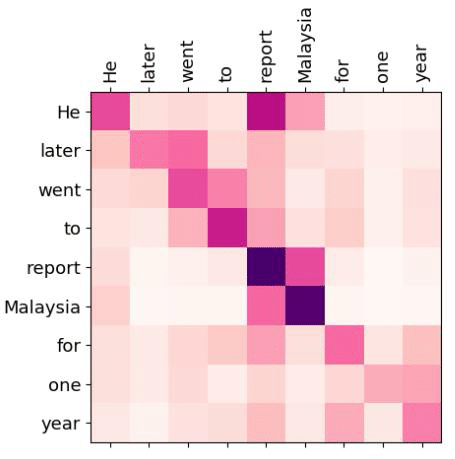
\includegraphics[width=0.8\textwidth]{images/attn_mat_example.png}
            \end{center}
        \end{column}
        \begin{column}{0.4\textwidth}
            \begin{itemize}
                \item Visualisation des scores d'attention entre tokens
                \item Chaque ligne représente l'attention d'un token vers tous les autres
                \item Les zones plus foncées indiquent une attention plus forte
                \item Permet d'interpréter quelles parties du texte sont liées
                \item Révèle les relations grammaticales et sémantiques capturées
            \end{itemize}
        \end{column}
    \end{columns}
\end{frame}


% Slide 17: Multi-Head Attention
\begin{frame}{Multi-Head Attention: Attention parallèle à plusieurs niveaux}
    \begin{columns}
        \begin{column}{0.4\textwidth}
            \begin{center}
                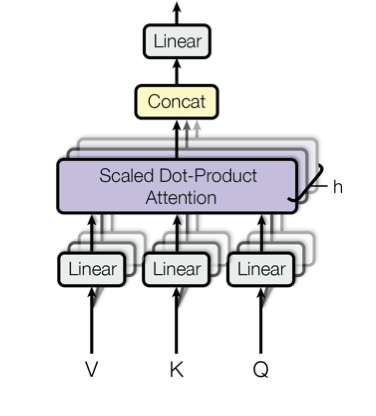
\includegraphics[width=\textwidth]{images/multi_head.png}
            \end{center}
        \end{column}
        \begin{column}{0.6\textwidth}
            \begin{align*}
                \text{MultiHead}(Q, K, V) &= \text{Concat}(\text{head}_1, ..., \text{head}_h)W^O \\
                \text{où head}_i &= \text{Attention}(QW^Q_i, KW^K_i, VW^V_i)
            \end{align*}
            \begin{itemize}
                \item Plusieurs "têtes" d'attention en parallèle
                \item Chaque tête se spécialise sur des aspects différents
                \begin{itemize}
                    \item Syntaxe, sémantique, coréférence, etc.
                \end{itemize}
                \item GPT-2 utilise 12 têtes, GPT-3 jusqu'à 96 têtes
                \item Les sorties des têtes sont concaténées puis projetées
                \item Permet de capturer plusieurs types de relations simultanément
            \end{itemize}
        \end{column}
    \end{columns}
\end{frame}

% Slide: Architecture du Transformer original
\begin{frame}{Architecture du Transformer: Le modèle original encoder-decoder}
    \begin{columns}
        \begin{column}{0.5\textwidth}
            \begin{center}
                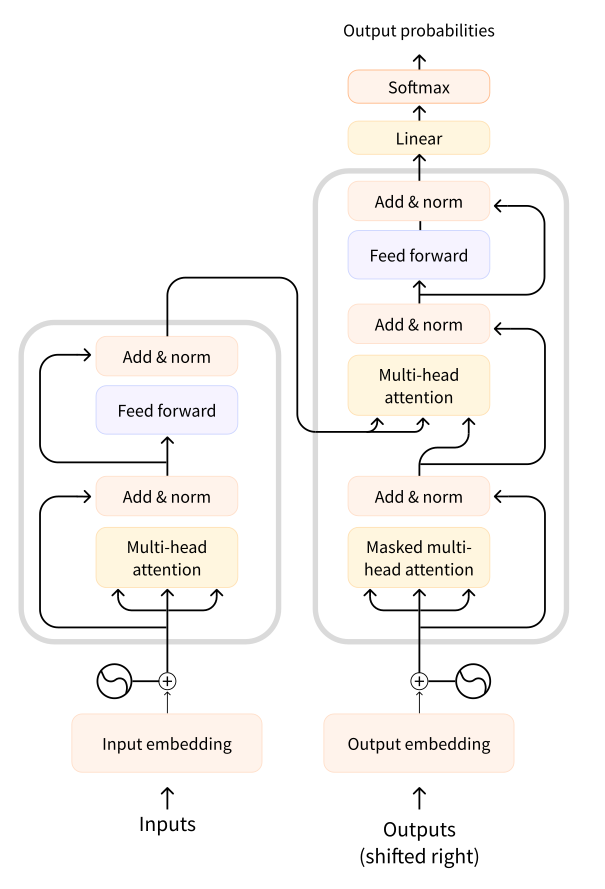
\includegraphics[width=0.6\textwidth, keepaspectratio]{images/transformers.png}
            \end{center}
        \end{column}
        \begin{column}{0.5\textwidth}
            \begin{itemize}
                \item \textbf{Architecture encoder-decoder}:
                \begin{itemize}
                    \item \textbf{Encoder}: Traite le texte source
                    \item \textbf{Decoder}: Génère le texte cible
                \end{itemize}
                \vspace{0.2cm}
                \item \textbf{Composants clés}:
                \begin{itemize}
                    \item Multi-head attention
                    \item Feed-forward networks
                    \item Residual connections
                    \item Layer normalization
                \end{itemize}
                \vspace{0.2cm}
                \item \textbf{Caractéristiques}:
                \begin{itemize}
                    \item Traitement parallèle des tokens
                    \item Attention bidirectionnelle (encoder)
                    \item Attention masquée (decoder)
                    \item Base de tous les modèles modernes
                \end{itemize}
            \end{itemize}
        \end{column}
    \end{columns}
\end{frame}

% Slide 18: Post-Attention et MLP
\begin{frame}{Après l'attention: Feed-Forward Network}
    \begin{columns}
        \begin{column}{0.4\textwidth}
            \begin{center}
                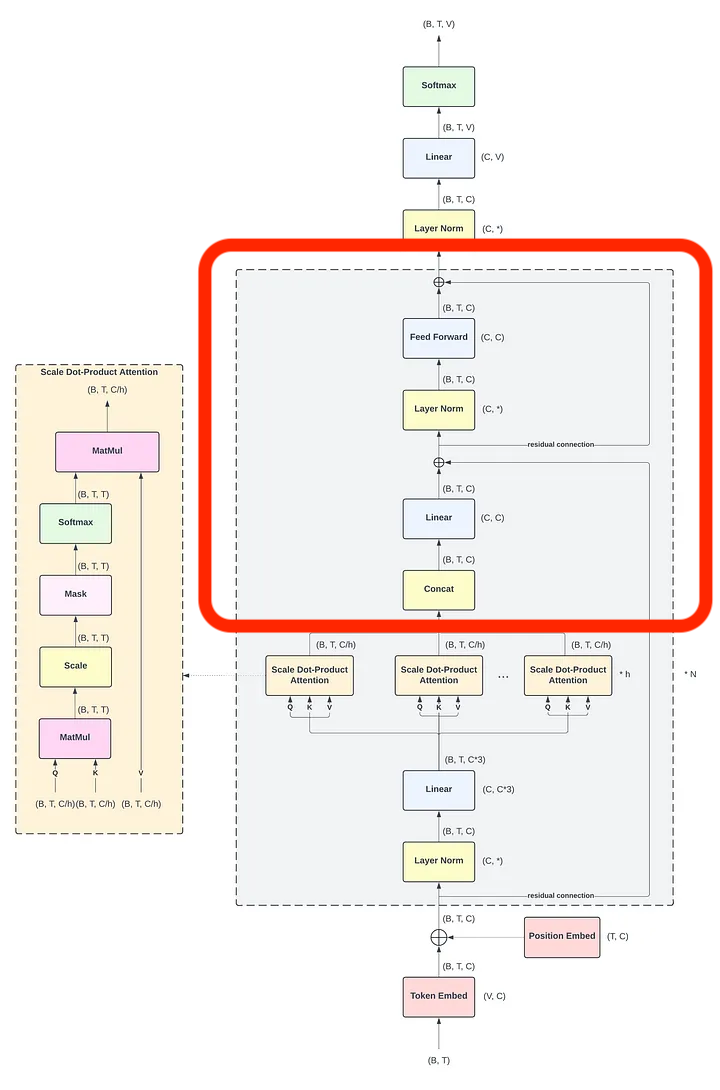
\includegraphics[width=0.8\textwidth]{images/post_attn.png}
            \end{center}
        \end{column}
        \begin{column}{0.6\textwidth}
            \begin{itemize}
                \item Après le mécanisme d'attention, vient un réseau feed-forward
                \item Appliqué indépendamment à chaque position (token)
                \item Composé de deux transformations linéaires et d'une activation
                \item Permet de transformer les représentations contextualisées
                \item Augmente la capacité de modélisation non-linéaire du réseau
                \item Contient la majorité des paramètres du Transformer
            \end{itemize}
        \end{column}
    \end{columns}
\end{frame}

% Slide 19: Structure détaillée du MLP
\begin{frame}{Structure du MLP dans les Transformers}
    \begin{center}
        \begin{tikzpicture}[>=latex, node distance=1.5cm, scale=0.65, transform shape]
            % Title for linear layer
            \node[text width=12cm, align=center] at (3,1) {\textbf{Projection linéaire dans le Feed-Forward Network}};
            
            % Inputs (reduced to 2)
            \foreach \i in {1,...,2}
            {
                \node (Input-\i) at (0,-\i*2) {$x_\i$};
            }

            % Hidden Layer
            \foreach \i in {1,...,6}
            {
                \node[draw, circle, minimum size=1cm] (Hidden-\i) at (3,{-\i*1.1+1}) {$f$};
            }

            % Output Layer (reduced to 2)
            \foreach \i in {1,...,2}
            {
                \node (Output-\i) at (6,-\i*2) {$y_\i$};
            }
            
            % Draw connections from inputs to the hidden layer and to the output layer
            \foreach \i in {1,...,2}
            {
                \foreach \j in {1,...,6}
                {
                    \draw[->] (Input-\i) -- (Hidden-\j);
                    \draw[->] (Hidden-\j) -- (Output-\i);
                }
            }

        \end{tikzpicture}
    \end{center}
    \vspace{-0.5cm}
    \begin{itemize}
        \item \textbf{Expansion}: La dimension cachée est 4 fois plus grande que l'entrée/sortie
        \item \textbf{GELU}: Fonction d'activation non-linéaire plus performante que ReLU
        \item \textbf{Projection}: Retour à la dimension d'origine
        \item \textbf{Dropout}: Régularisation pour éviter le surapprentissage
    \end{itemize}
\end{frame}

\end{document}
